\documentclass [a4paper,12pt]{article}
\usepackage[left = 2.5cm, rigth = 2.5cm, top = 3cm, bottom = 3 cm] {geometry}
\usepackage{amsmath,amsthm,amssymb}
\usepackage{cite}
\usepackage{url}
\usepackage[utf8]{inputenc}
\usepackage[spanish]{babel}
\usepackage{graphicx}
\bibliographystyle{plain}

\begin{document}
\title{Presentación Moogle!}
\author{Abel Ponce Gonzalez}
\date{Julio, 2023}
\maketitle
\newpage
\begin{figure}[h]
	\center
	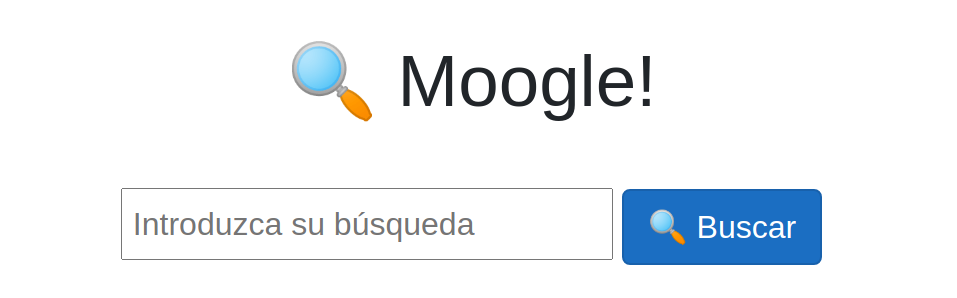
\includegraphics[width = 15cm]{moogle.png}
	\label{fig:moogle}
\end{figure}
Es un motor de búsqueda que dado una query que introduzca el usuario, devuelve los resultados más relevantes de dicha búsqueda en la base de datos asignada en la carpeta Content.
\section{Objetivo}\label{sec:objetivos}
El objetivo es realizar búsquedas en el interior de los txt pertenecientes a la base de datos y en función de esto mostrar los resultados más relevantes con respecto a la búsqueda.
\section{Ejecución}\label{sec:ejecucion}
\subsection{Paso \texttt{1}}\label{sub:center}
\begin{figure}[h]
	\center
	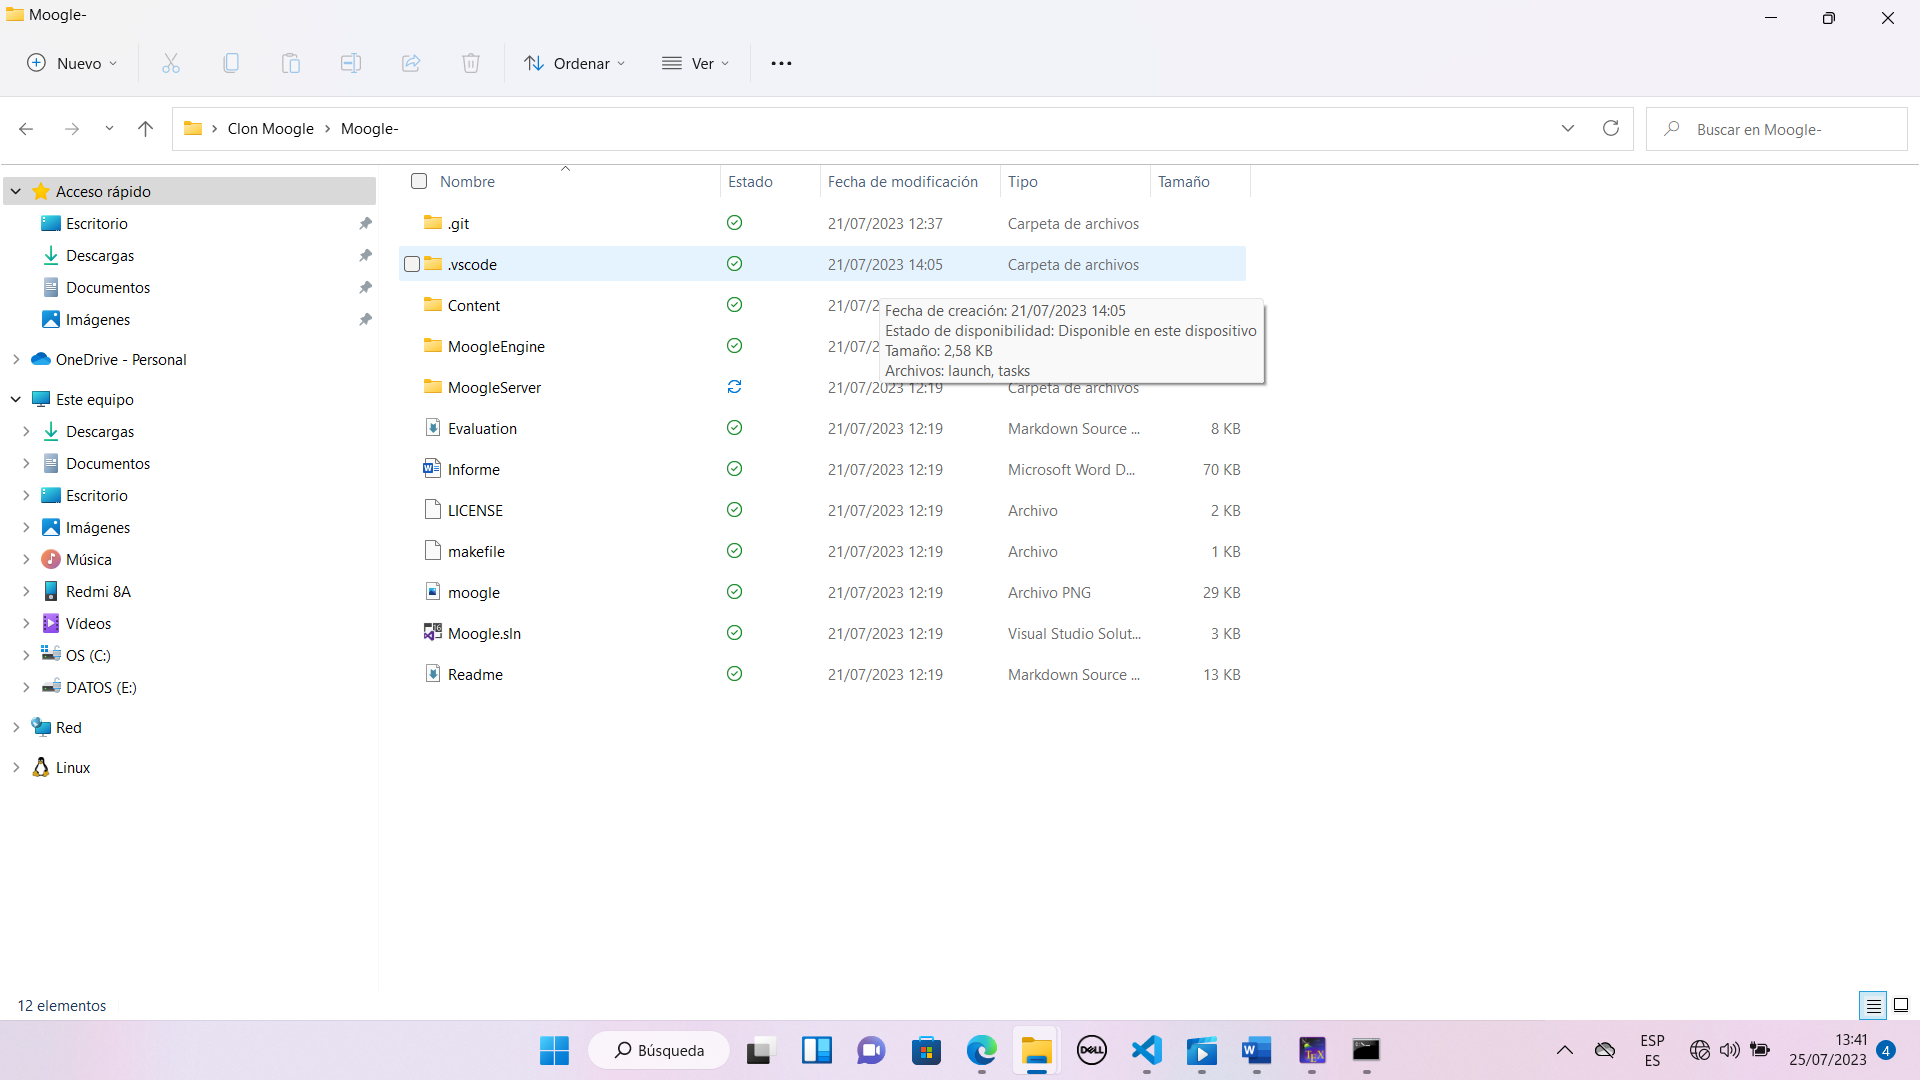
\includegraphics[width = 14cm]{Carpeta.png}
	\label{fig:carpeta}
\end{figure}
Abrir la carpeta donde se encuentra el proyecto
\subsection{Paso \texttt{2}}\label{sub:center}
\begin{figure}[h]
	\center
	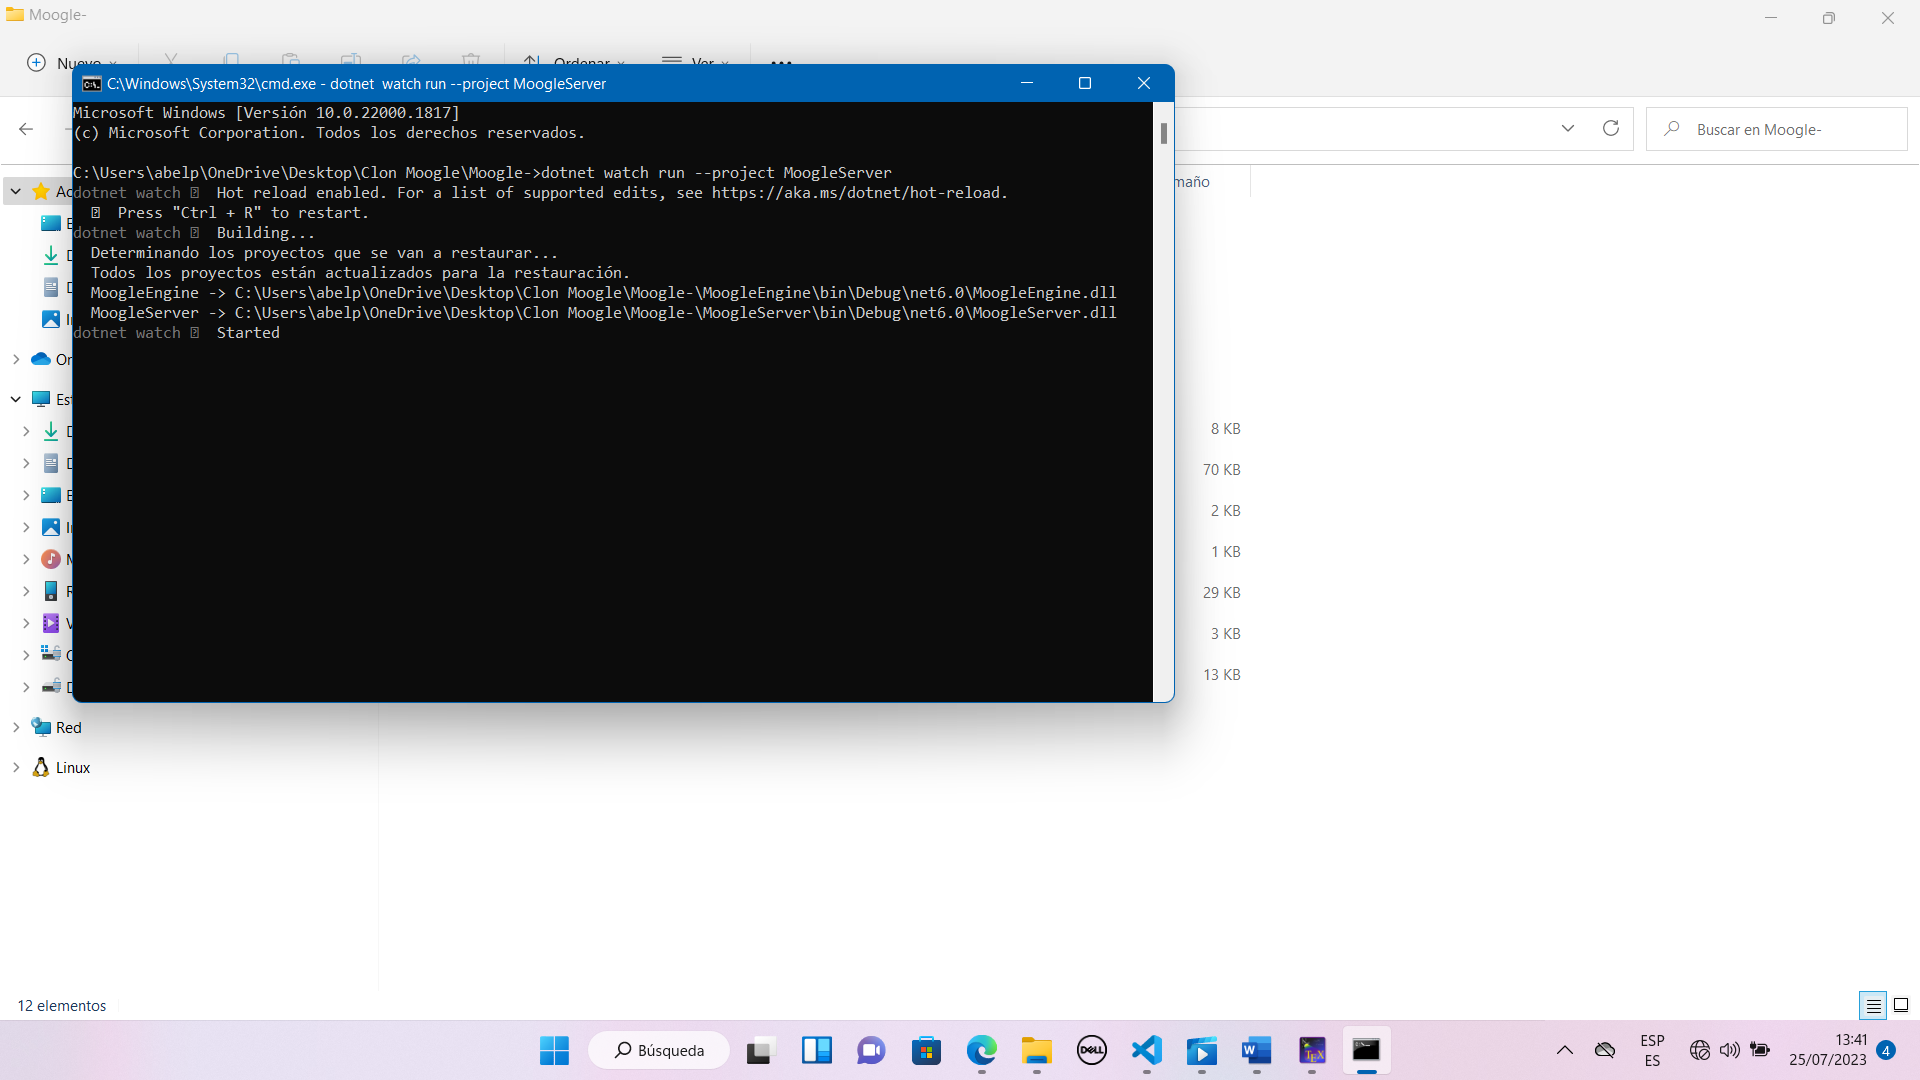
\includegraphics[width = 14cm]{Terminal.png}
	\label{fig:terminal}
\end{figure}
Abrir la terminal y escribir el siguiente comando:
dotnet watch run --project MoogleServer
\subsection{Paso \texttt{3}}\label{sub:center}
\begin{figure}[h]
	\center
	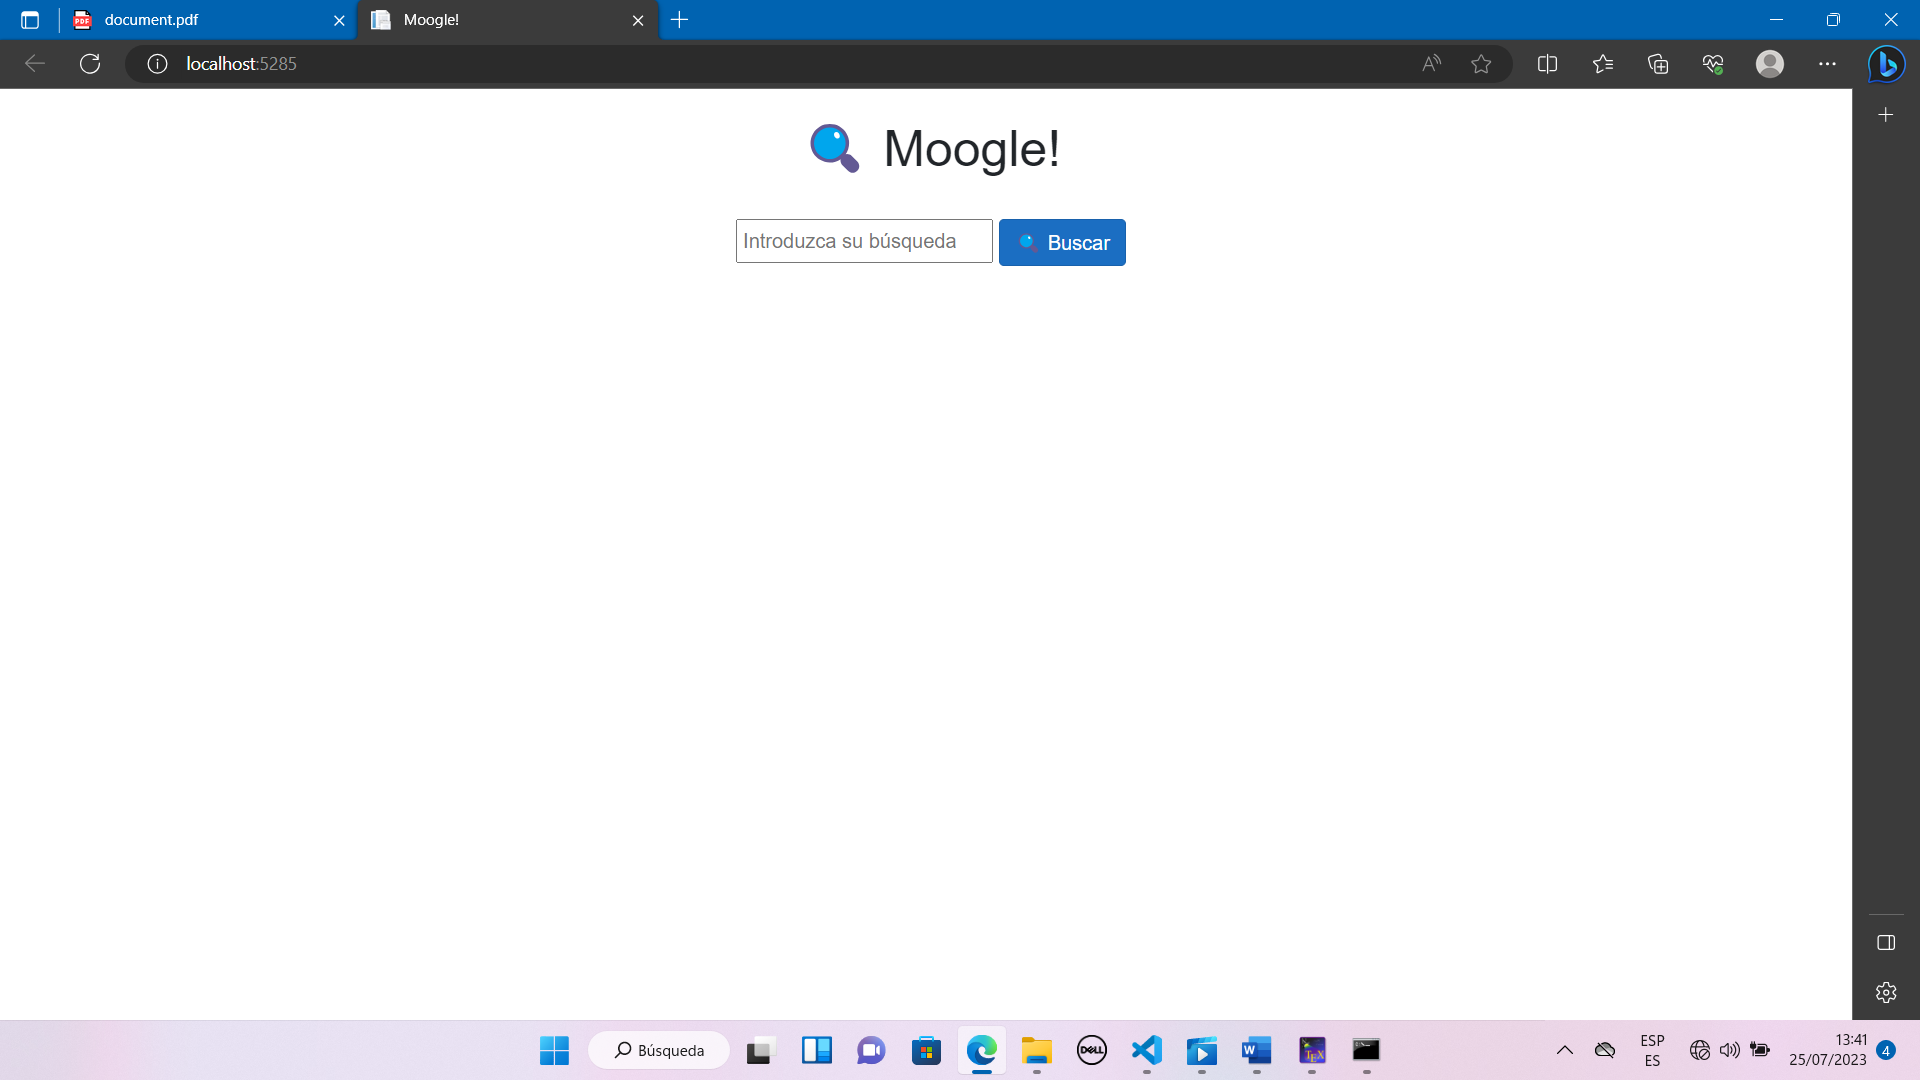
\includegraphics[width = 14cm]{Navegador.png}
	\label{fig:navegador}
\end{figure}
Abrir en el navegador la dirección que ofrece
\newpage
\section{Algoritmo}\label{sec:algoritmo}
En este proyecto implemente una clase llamada documentos donde estaría la mayor parte del algoritmo, a la cual le di propiedades entre ellas están: archivos (posee las rutas de cada txt de la base datos), textos (posee cada texto de la base sin signos de puntuación), palabrasUnicas (lista de todas las palabras sin repetir), matriz (matriz numérica de TF-IDF). 
\subsection{Acerca \texttt{TF-IDF}}\label{sub:center}
A grandes rasgos la conversión se lleva acabo cuando a cada palabra se le hace corresponder su TF*IDF, el cual es especifico de cada una.
TF: Es la frecuencia de la palabra en todo el texto entre la cantidad de palabras total del este.
IDF: Es el logaritmo en base 2 cuyo argumento es la cantidad de documentos totales de la bases de datos entre la cantidad de documentos en los que aparece la palabra trabajada en ese momento. En el caso especifico de mi proyecto en el denominador le sume 0.001 ante el inminente miedo que la palabra no apareciera en ningún documento y se indefiniera la fracción.
\subsection{Sugerencia \texttt{Levenshtein}}\label{sub:center}
En el proyecto está implementada una vía para dar sugerencias al usuario a través del algoritmo de Levenshetein además de que puedes tocar el link de la sugerencia y t dará los resultados más relevantes de la búsqueda de la palabra.
\begin{figure}[h]
	\center
	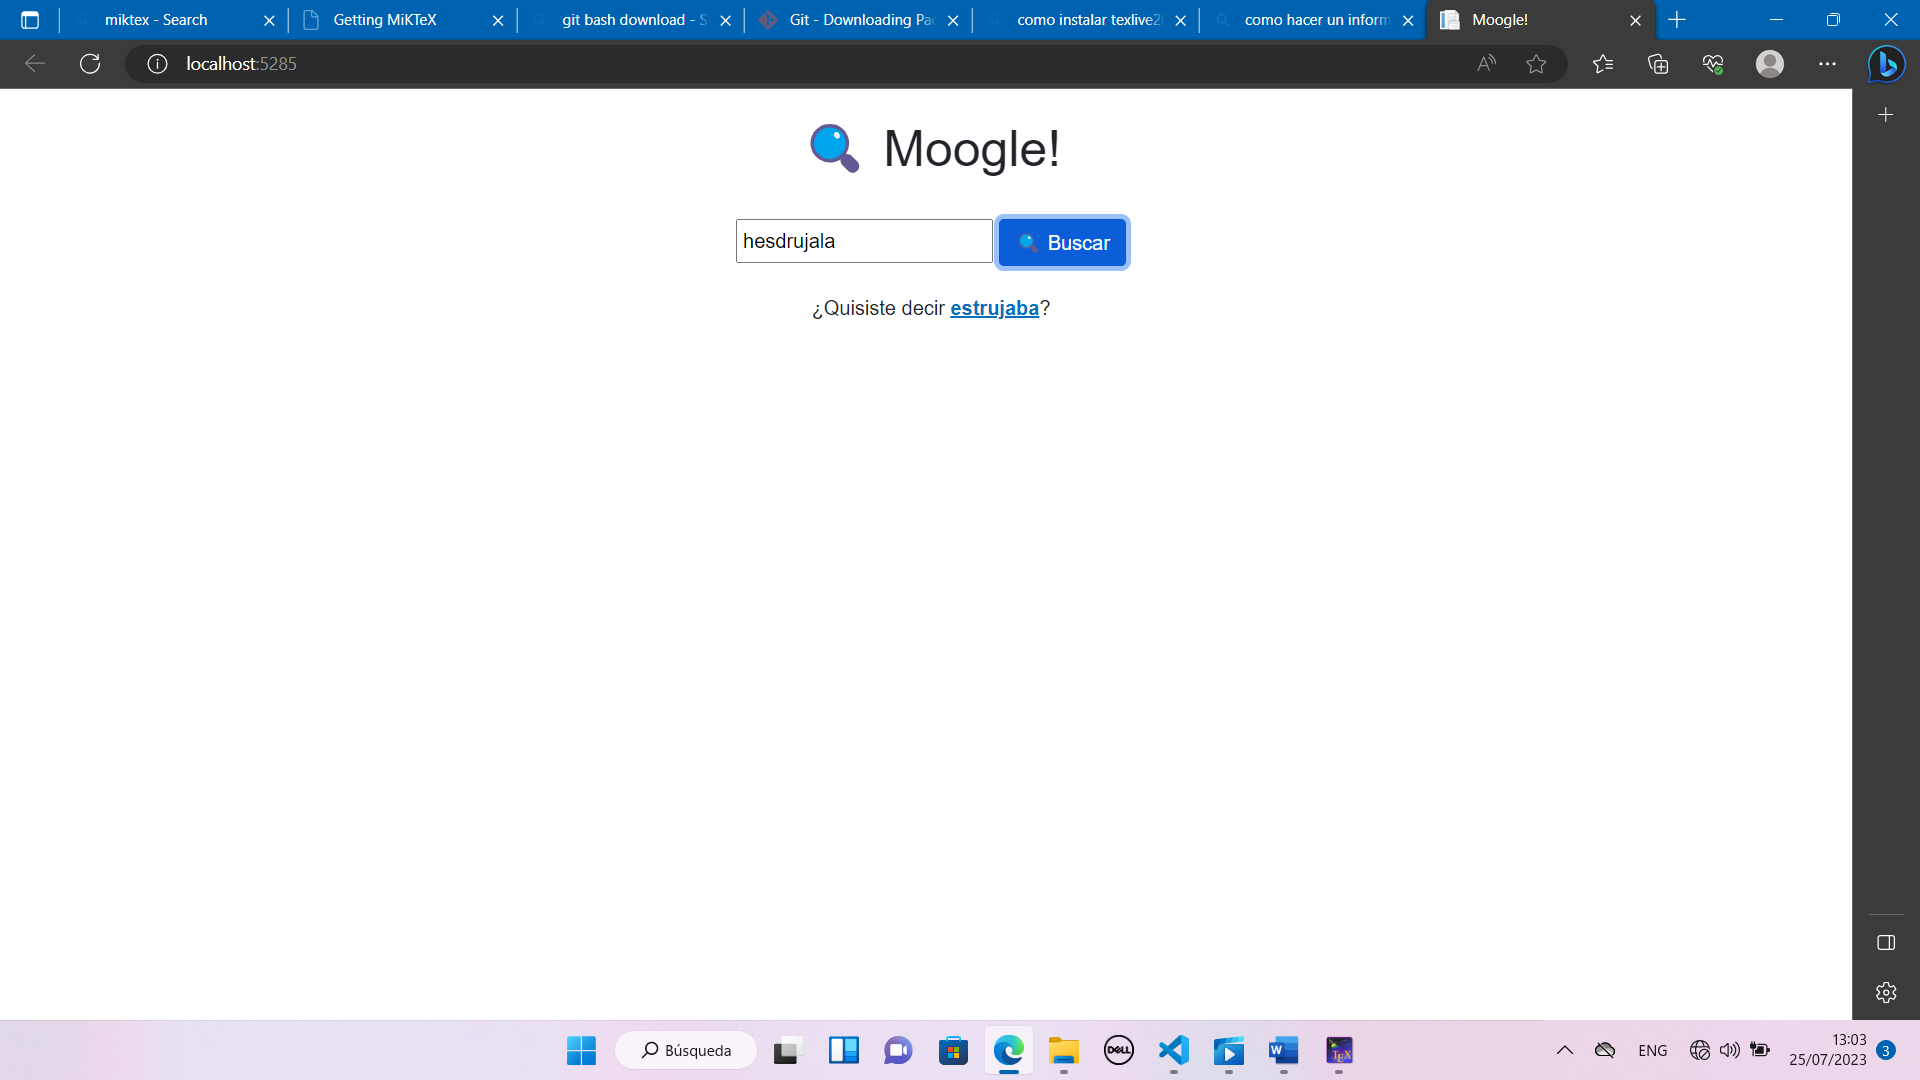
\includegraphics[width = 14cm]{sugerencia.png}
	\label{fig:navegador}
\end{figure}
\begin{figure}[h]
	\center
	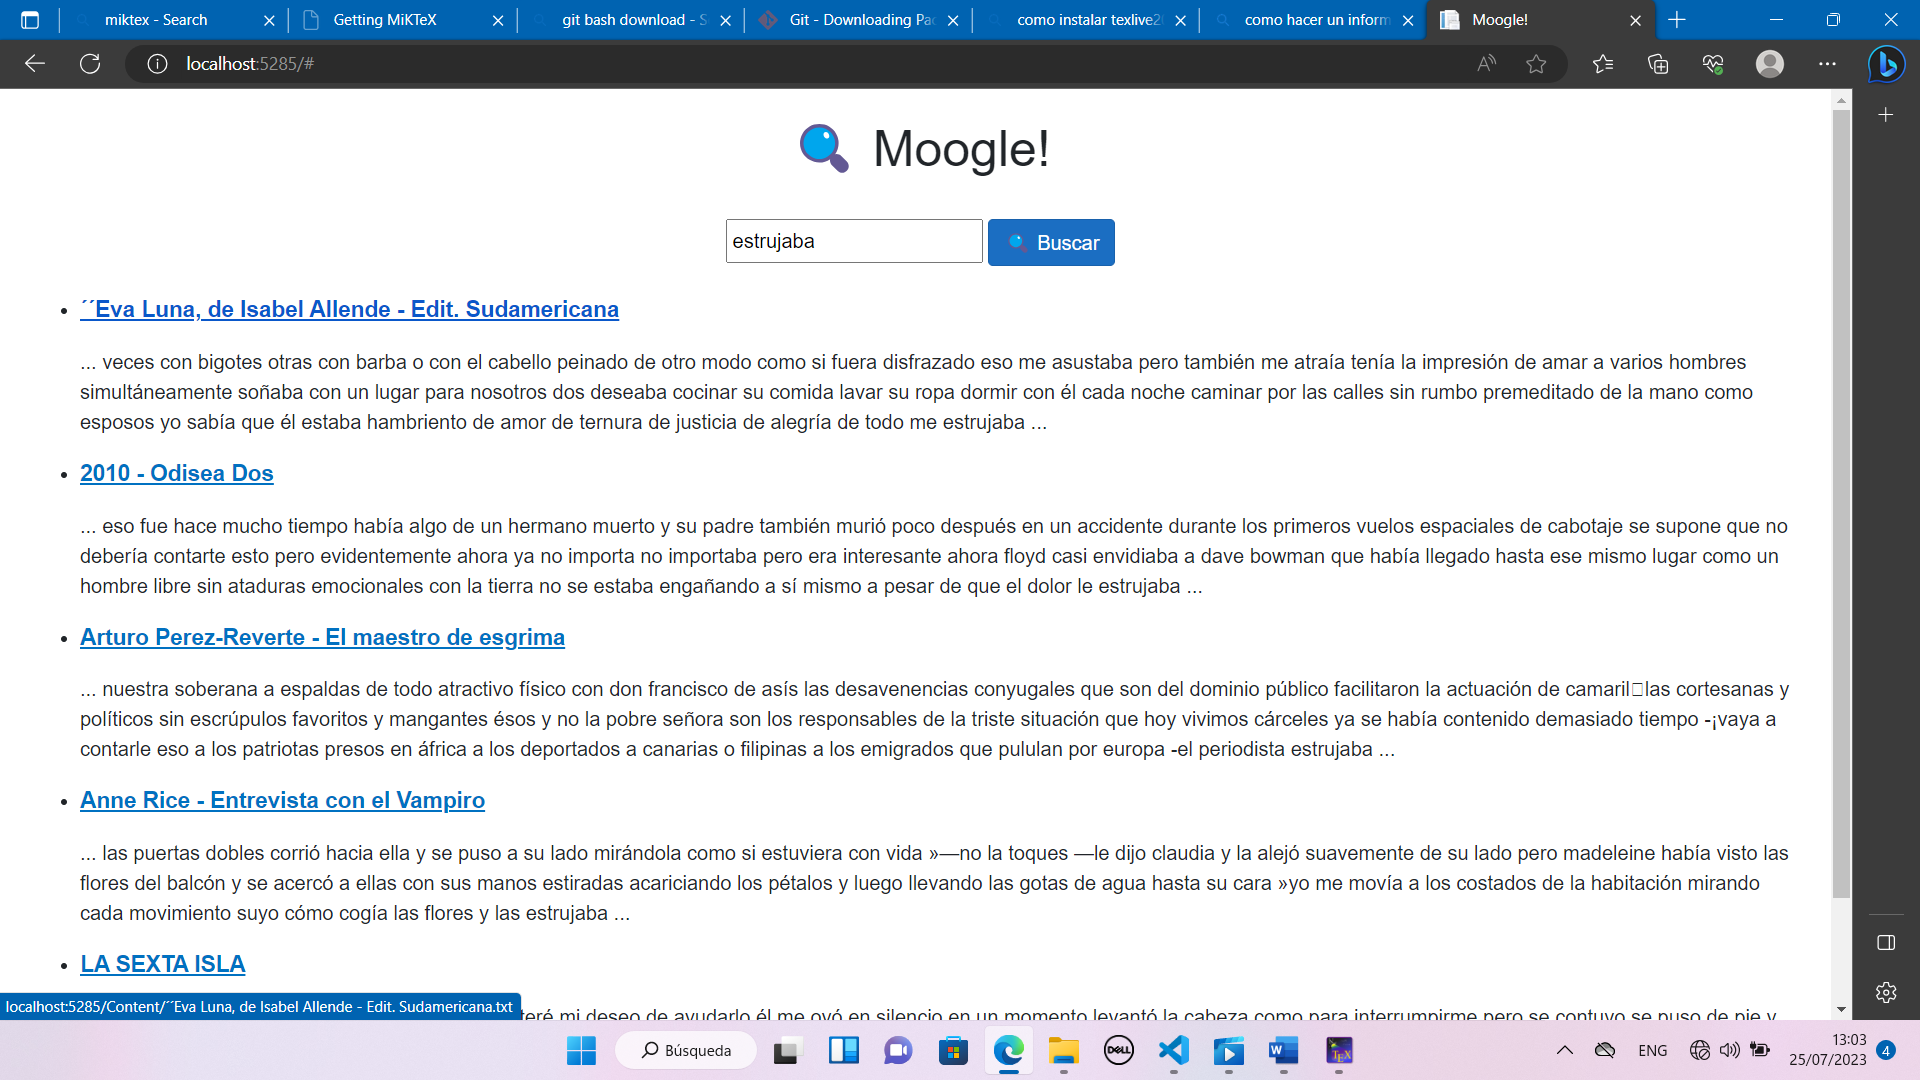
\includegraphics[width = 14cm]{buscada.png}
	\label{fig:navegador}
\end{figure}
\end{document}